% -*- coding: iso-8859-1 -*-
% !TeX spellcheck = de_DE
% !TeX encoding = iso-8859-1

\chapter{Umsetzung und Implementierung}
\label{ch:implementierung}

Zur Umsetzung des Projekts wurde uns von Seiten des Lehrstuhls ein GitLab-Repository mit integriertem Continuous-Integration-Server (CI-Server) zur Verfügung gestellt. Programmiert wurde in portablem und modernem C++ (im aktuellen Standard \textit{C++14}).  Außerdem haben wir uns für das Buildsystem \textit{cmake} und für die graphische Entwicklungsumgebung \textit{CLion} entschieden. Die meiste Zeit wurde via \textit{Teamviewer} mit der aus der agilen Softwareentwicklung bekannten Arbeitstechnik \textit{Paarprogrammierung} gearbeitet.

Ziel war es, kompatible Software für zwei vorgegebene Test- und Benchmark-Systeme zu entwickeln (im Folgenden \textit{i41pc189} und \textit{i41pc205} genannt). Die Anwendung wurde aber für alle gängigen Systeme ausgelegt; Programmcode und CMake-Konfiguration wurden so eingerichtet, dass nur für die aktuelle Umgebung kompatible Maschinenbefehle kompiliert werden (z.B. Abschalten von AVX bei fehlender Hardwareunterstützung).

Die einzigen von der Aufgabenstellung zugelassenen Bibliotheken waren:
\begin{itemize}[noitemsep,topsep=0pt,parsep=0pt,partopsep=0pt]
\item \url{https://github.com/nothings/stb} zum Schreiben von Bitmaps,
\item \url{https://nlohmann.github.io/json/} zum Lesen von JSON-Dateien,
\item \url{https://github.com/syoyo/tinyobjload} zum Laden von OBJ-Dateien
\end{itemize}
sowie die NVIDIA Bibliotheken \textit{CUDA} und \textit{Thrust} zur Programmierung der Grafikkarte (GPGPU-Programmierung).

\section{Software-Architektur}
Beide Aufgabenteile (Raytracing und Pathtracing) mussten in einer gemeinsamen Anwendung implementiert werden. Welches der beiden Tracing-Verfahren zum Einsatz kommt wird dabei dynamisch zur Laufzeit aus der Szenen-Beschreibung (JSON-Datei) ausgelesen. Da anfangs noch mit Anpassungen und Erweiterungen der Aufgabenstellung zu rechnen war, entschieden wir uns für einen möglichst modularen und objektorientierten Software-Entwurf. Eine Auflistung und Beschreibung der entwickelten Module findet sich in \autoref{tbl:moduls}. 

Der Programmablauf ließ sich in die folgenden Schritte untergliedern:
\begin{enumerate}
\item Dateieingabe: Lesen der Szenen-Beschreibung (JSON) und Obj-Datei
\item Vorverarbeitung der Szene: Vorberechnungen für die Dreiecke (z.B. Berechnung der Normalen), Konstruieren des k-d-Baums und Berechnung der Primärstrahlen; in diesem Schritt werden auch anhand der Szene Weichen für das weitere Vorgehen gestellt (Wahl des k-d-Baums, Entscheidung, ob GPU verwendet werden soll)
\item Rendering: Durchführung des Tracing-Verfahrens
\item Dateiausgabe: Schreiben des Ergebnisbildes in eine Bitmap-Datei
\end{enumerate}

\begin {table}[htbp]
	\begin{center}
    \begin{tabular}{ | l | p{10cm} |}
    \hline
    \textbf{Modulname} & \textbf{Beschreibung} \\ \hline
    main.h & Einstiegspunkt mit Mainfunktion; verbindet die Komponenten miteinander und misst deren Ausführungszeiten. \\ \hline
    options.h & Datei zum Setzen verschiedenerer statischer Programmparameter; zum Ein- und Ausschalten von AVX, SSE und CUDA. \\ \hline
    io.h & Zuständig für das Parsen der JSON-Szenen-Beschreibung und der Wavefront OBJ-Datei.\\ \hline
    scene\_preprocessor.h & Vorverarbeitung der Szene (siehe oben). \\ \hline
    pray.h & Mit dem Aufruf von \texttt{render(...)} wird das Tracing-Verfahren gestartet; die Entscheidung ob Ray- oder Pathtracing durchgeführt wird, wird anhand der Informationen aus dem Szene-Objekt (Parameter) entschieden. \\ \hline
    geometry.h & Definiert die benötigten geometrischen Primitiven (\textit{Vec3}, \textit{Triangle}, \textit{Bounding Box}, usw.) und die auf ihnen ausgeführten Algorithmen (z.B. Dreieck- und BB-Schnitt). \\ \hline
    geometry\_simd.h & Erweitert die Algorithmen aus \textit{geometry.h} um deren SSE und AVX Pendants (Intrinsics). \\ \hline
    spatial.h  & \multirow{4}{*}{\parbox{10cm}{Schnittstelle für räumliche Datenstrukturen und die\newline dazugehörigen Instanziierungen (siehe \autoref{sec:spatial}).}} \\ 
    bf\_search.h & \\
    kd\_tree.h & \\ 
    kd\_tree\_sah.h & \\ 
    kd\_tree\_hybrid.h & \\ \hline
	path\_trace.cu.h & \multirow{4}{*}{\parbox{10cm}{CUDA-Code für paralleles Pathtracing auf der GPU.}} \\
    kd\_tree\_gpu.h & \\
    gpu\_util.h & \\ \hline
    \end{tabular}
    \caption {Beschreibung der Module}
    \label{tbl:moduls}
	\end{center}
\end {table}

\section{Implementierung der räumlichen Datenstruktur}\label{sec:spatial}
Es wurde schnell klar, dass die Schnittberechnung der Dreiecke mit den Strahlen der Flaschenhals der Laufzeit werden würde. Um hier möglichst einfach zwischen alternativen räumlichen Datenstrukturen wechseln zu können, entschieden wir uns für eine Vererbungshierarchie wie in \autoref{img:spatial} dargestellt.

\begin{figure}[htbp]
	\centering
	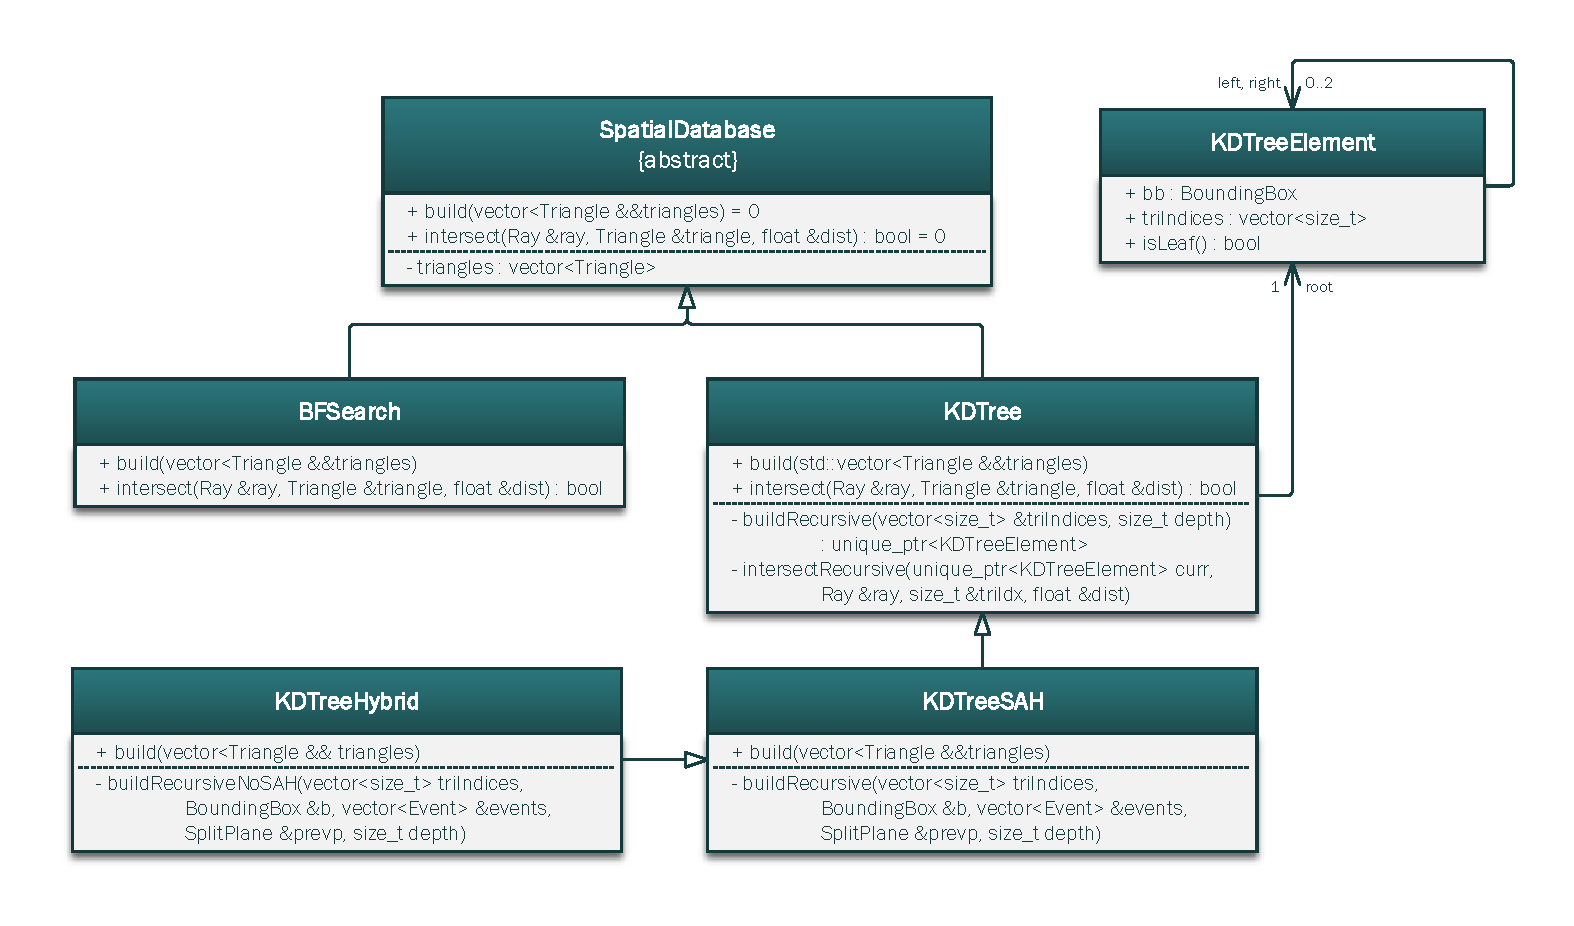
\includegraphics[width=1\textwidth]{graphics/spatial.pdf}
	\caption{Klassendiagramm: Räumliche Datenstruktur}
	\label{img:spatial}
\end{figure}

Die Klasse \texttt{SpatialDatabase} stellt zwei abstrakte Methoden \texttt{build} und \texttt{intersect} bereit. Diese werden dann von den Unterklassen \texttt{BFSearch} und \texttt{KDTree} implementiert. \texttt{BFSearch} führt bei der Schnittberechnung eine vollständige Suche über alle Dreiecke durch. Beim bauen wird lediglich ein \textit{move} aller Dreiecke in die Instanzvariable \textit{triangles} vorgenommen.
In \texttt{KDTree} wird in \texttt{build} ein naiver k-d-Baum aufgebaut. \texttt{KDTreeSAH} erzeugt k-d-Bäume gemäß der Surface-Area-Heuristik. Die Schnittberechnung von \texttt{KDTreeSAH} wird von  \texttt{KDTree} geerbt.

Der Aufbau der beiden k-d-Bäume erfolgt rekursiv und wurde wie in \autoref{sec:openmp} beschrieben mit \textit{OpenMP}-Tasks parallelisiert. Neue Tasks werden jedoch nur bis zu einer bestimmten Tiefe \textbf{TASK\_DEPTH} erzeugt. Die maximale Tiefe des konstruierten Baums und die Mindestzahl benötigter Dreiecke für einen weitere Teilung sind durch die beiden Parameter \textbf{MAX\_DEPTH} und \textbf{THRESHOLD} beschränkt.
Für die Konstruktion des Baums mit SAH wurde zunächst der Algorithmen in $\mathcal{O}(n\log^2{}n)$\ aus \cite{wald2006building} implementiert. Später wurde dann zur Beschleunigung ein Wechsel auf den $\mathcal{O}(n\log{}n)$-Algorithmus vorgenommen.

\section{Implementierung des Raytracers}
Der Raytracer wurde zunächst in einer möglichst einfachen, sequentiellen Variante entworfen. Der Dreiecksschnitt wurde von Anfang an mit dem Möller–Trumbore-Schnitt\-algorithmus durchgeführt. Im nächsten Schritt wurde die vollständige Suche nach dem Dreieck mit geringstem Abstand durch eine wesentliche effizientere Suche in einem k-d-Baum ersetzt (siehe \autoref{sec:kdTree} und \autoref{sec:spatial}). Der erste Ansatz zur Parallelisierung war eine Verteilung der Bildpixel/Primärstrahlen auf mehrere Threads. Da hierbei keine Abhängigkeiten zwischen Pixeln existieren (\textit{embarrassingly parallel}), konnte dies auf einfache Weise mit OpenMP vorgenommen werden.
Eine weitere Beschleunigung konnte anschließend durch die Bündelung von Strahlen erreicht werden (siehe \autoref{sec:ray_tracer}). Da die Testmaschine \textit{i41pc205} keine AVX-Instruktionen unterstützt, entschieden wir uns dafür, abhängig von der Zielplattform, unser Programm sowohl für SSE (vier Strahlen) als auch für AVX (acht Strahlen) zu optimieren. Da jeder Prozessor seine eigenen SIMD-Register besitzt, skaliert dieser Ansatz auch äußerst gut mit der vorherigen Parallelisierung mit \textit{OpenMP}. Um auf die hardwarenahen SIMD-Instruktionen zurückzugreifen, wurden intrinsische Funktionen (Intrinsics) verwendet. Hierzu musste der Möller-Trumbore-Algorithmus für SIMD umgeschrieben werden und es waren Anpassungen in der k-d-Baum Schnittberechnung erforderlich.

\section{Implementierung des Pathtracers}
Eine erste Version des Pathtracers konnte durch nur wenige Anpassungen am schon vorhandenen Raytracer implementiert werden. Es zeigte sich jedoch, dass aufgrund der mit der Rekursionstiefe exponentiell wachsenden Anzahl Strahlen eine reine Parallelisierung über die Pixel zu unzufriedenstellenden Laufzeiten führt.
Wie in \autoref{sec:path_tracer} beschrieben ist eine Parallelisierung des Pathtracings mit den SIMD-Registern der CPU nur eingeschränkt sinnvoll.
Um das Tracing auf der GPU durchführen zu können mussten viele der schon vorhandenen Funktionen aus \texttt{geometry.h} in CUDA-Kernel-Code überführt werden. Außerdem muss der k-d-Baum in eine für die GPU besser geeignete Form umkopiert werden. Bei der Implementierung des Verfahrens in CUDA kam es zu mehreren Schwierigkeiten: 
\begin{itemize}
\item Da das Programmiermodell von Grafikkarten nicht für rekursive Funktionsaufrufe ausgelegt ist, versuchten wir in unserem ersten Lösungsansatz diese aus dem Programmcode zu eliminieren. Dazu mussten in einem Array alle Strahlen (über alle Pixel) auf der momentanen Rekursionstiefe zwischengespeichert werden. Dieser Ansatz musste später aufgrund eines zu hohen Speicherverbrauches (sowohl auf der GPU als auch auf der CPU) verworfen werden.
\item Bei der rekursiven Variante kam es ebenfalls zu Problemen mit dem GPU-Speicher. Hier kommt es zu einer zweifachen Rekursion: Einerseits die beim Pathtracing vorgebenene Rekursion beim Auftreffen auf ein Dreieck, andererseits der rekursive Abstieg auf dem k-d-Baum für die Schnittberechnung. Eine \glqq Stackless\grqq-Traversierung (siehe \cite{popov2007stackless}) des k-d-Baum gestaltete sich als deutlich schwieriger zu implementieren als zunächst erwartet.
\item Eng verwandt mit dem vorherigen Punkt ist die Festellung, dass ein k-d-Baum der gemäß der SAH-Metrik aufgebaut wurde, nur eingeschränkt für die GPU geeignet ist. SAH neigt dazu deutlich tiefere Bäume zu erzeugen, was bei der Traversierung zu einer größeren Rekursionstiefe führt. Mit einem naiven k-d-Baum konnten teilweise deutlich bessere Laufzeiten erzielt werden. Um ein gutes Mittelmaß bei den Laufzeiten zu finden, wurde eine SAH-Abwandlung eingeführt, welche auf den ersten Ebenen die naive Unterteilungsmetrik verwendet und erst dann auf SAH wechselt. Siehe \texttt{KDTreeHybrid} in \ref{img:spatial}.
\end{itemize}

Da andere Gruppen beim Pathtracing deutlich geringere Laufzeiten erzielten als unsererer Meinung nach mit dem vorgeschriebenem Algorithmus (auch als \textit{diffuses Raytracing} bezeichnet) möglich ist, wurde ebenfalls noch eine etwas abgewandelte Variante des Verfahrens implementiert. Bei dem in \autocite{Kajiya:1986:RE:15886.15902} vorgestellten Algorithmus zum Pathtracing wird nicht bei jedem Treffer auf ein Objekt ein neuer Strahl erzeugt, stattdessen wird \textbf{NUM\_SAMPLES} oft über jedes der Pixel iteriert und jeweils nur ein Pfad verfolgt. Am Ende wird der berechnete Pixelwert dann durch \textbf{NUM\_SAMPLES} geteilt. Dies führt zu vergleichbaren Ergebnisbildern, erzeugt aber bei Rekursionstiefen größer eins deutlich weniger Strahlen; die Anzahl der Strahlen ist linear und nicht exponentiell zu \textbf{NUM\_SAMPLES}.




